\documentclass[tikz,border=5mm]{standalone}
\usetikzlibrary{arrows.meta, positioning}

\tikzset{
  block/.style={rectangle, draw, rounded corners,
                minimum width=5cm, minimum height=1cm,
                align=center},
  arrow/.style={-{Latex[length=3mm]}, thick}
}

\begin{document}
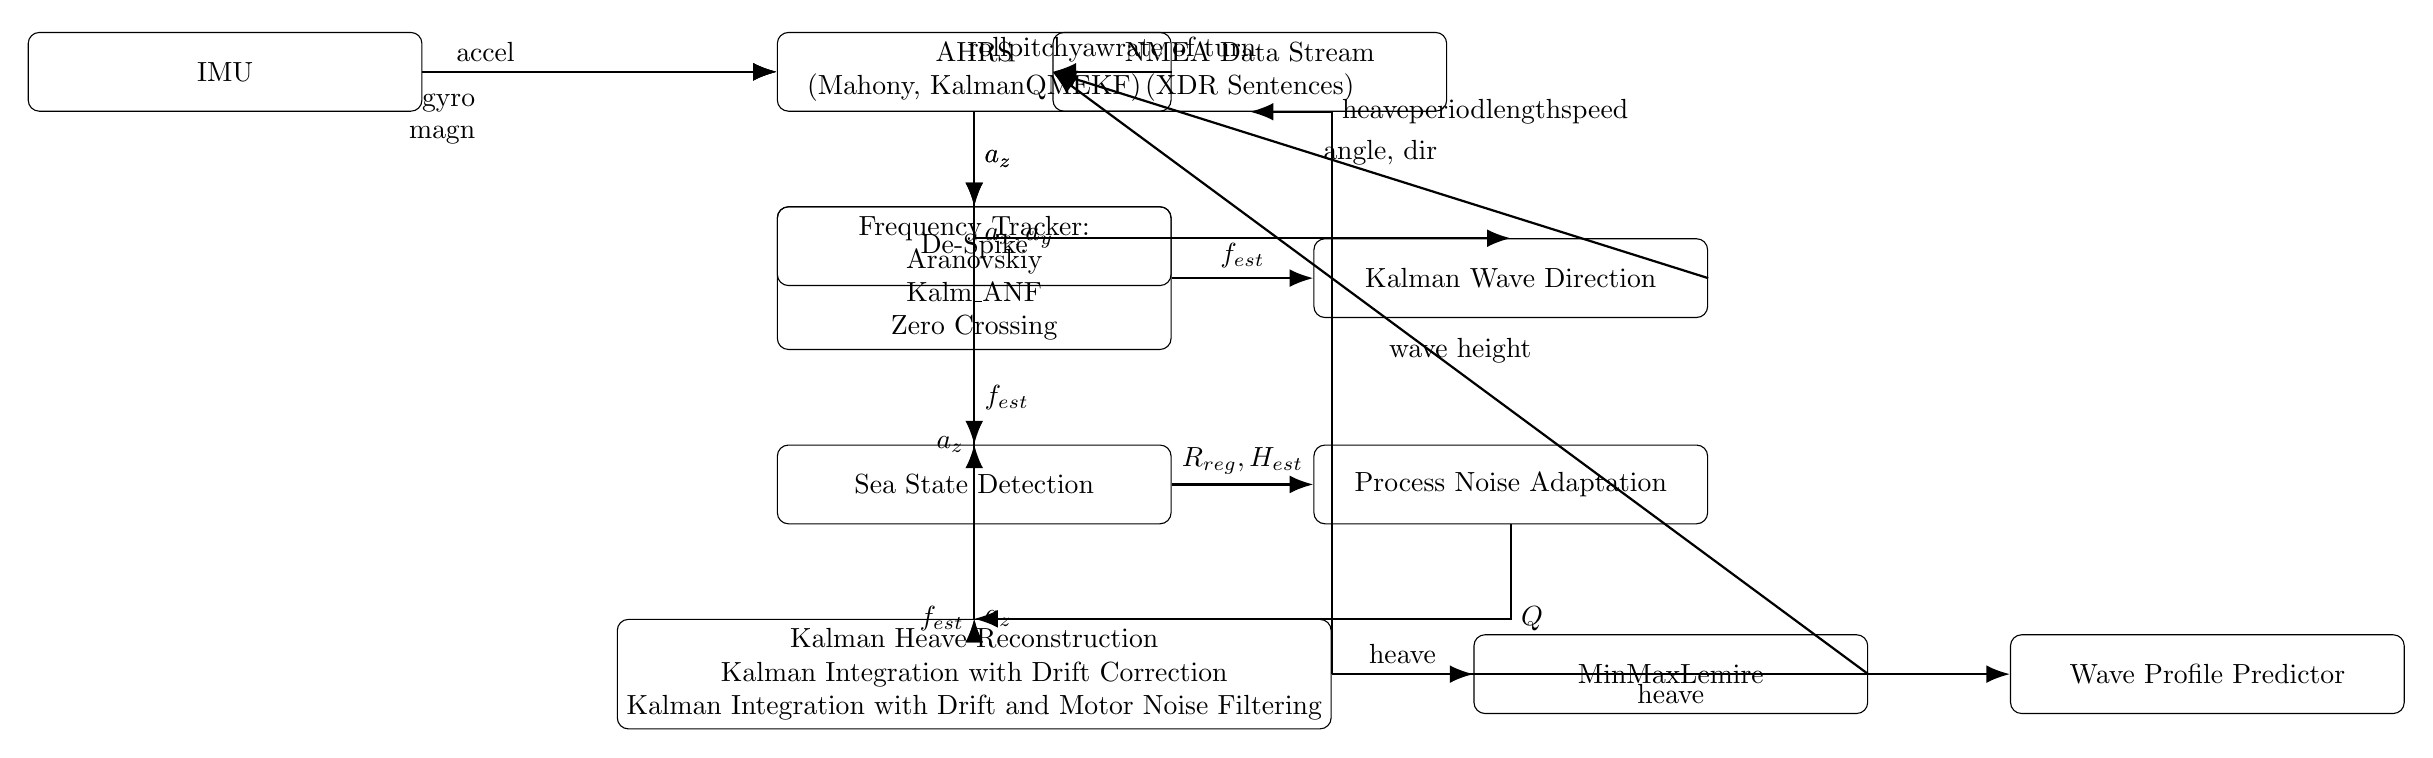
\begin{tikzpicture}[node distance=1.2cm and 1.8cm]

% Row 1: IMU + AHRS + NMEA
\node[block] (IMU) {IMU};
\node[block, right=4.5cm of IMU] (AHRS) {AHRS\\(Mahony, KalmanQMEKF)};
\node[block, right=8cm of IMU] (NMEA) {NMEA Data Stream\\(XDR Sentences)};

% Row 2: Frequency tracker + Wave Direction
\node[block, below=of AHRS] (FreqTracker) {Frequency Tracker:\\Aranovskiy\\Kalm\_ANF\\Zero Crossing};
\node[block, right=of FreqTracker] (WaveDir) {Kalman Wave Direction};

% Row 3: Sea State + Noise Adapt
\node[block, below=of FreqTracker] (SeaReg) {Sea State Detection};
\node[block, right=of SeaReg] (NoiseAdapt) {Process Noise Adaptation};

% Row 4: Kalman Heave + MinMax + Predictor
\node[block, below=of SeaReg] (KalmanWave) {Kalman Heave Reconstruction\\
Kalman Integration with Drift Correction\\
Kalman Integration with Drift and Motor Noise Filtering};
\node[block, right=of KalmanWave] (MinMax) {MinMaxLemire};
\node[block, right=of MinMax] (WavePredictor) {Wave Profile Predictor};

% Row 2.5: DeSpike under AHRS
\node[block, below=of AHRS] (DeSpike) {De-Spike};

% --- Connections ---
% IMU -> AHRS
\draw[arrow] (IMU.east) -- ++(0.8,0) |- (AHRS.west) node[midway,above] {accel};
\draw[arrow] (IMU.east) -- ++(0.8,0) |- (AHRS.west) node[midway,left,yshift=-4mm] {gyro};
\draw[arrow] (IMU.east) -- ++(0.8,0) |- (AHRS.west) node[midway,left,yshift=-8mm] {magn};

% AHRS -> Frequency Tracker
\draw[arrow] (AHRS.south) -- (FreqTracker.north) node[midway,right] {$a_{z}$};

% Frequency Tracker -> SeaReg
\draw[arrow] (FreqTracker.south) -- (SeaReg.north) node[midway,right] {$f_{est}$};

% AHRS -> SeaReg
\draw[arrow] (AHRS.south) |- (SeaReg.north) node[midway,left] {$a_{z}$};

% AHRS -> WaveDir
\draw[arrow] (AHRS.south) |- (WaveDir.north) node[midway,right] {$a_{x},a_{y}$};

% FreqTracker -> WaveDir
\draw[arrow] (FreqTracker.east) -- (WaveDir.west) node[midway,above] {$f_{est}$};

% SeaReg -> NoiseAdapt
\draw[arrow] (SeaReg.east) -- (NoiseAdapt.west) node[midway,above] {$R_{reg},H_{est}$};

% FreqTracker -> KalmanWave
\draw[arrow] (FreqTracker.south) |- (KalmanWave.north) node[midway,left] {$f_{est}$};

% NoiseAdapt -> KalmanWave
\draw[arrow] (NoiseAdapt.south) |- (KalmanWave.north) node[midway,right] {$Q$};

% AHRS -> DeSpike -> KalmanWave
\draw[arrow] (AHRS.south) -- (DeSpike.north) node[midway,right] {$a_{z}$};
\draw[arrow] (DeSpike.south) |- (KalmanWave.north) node[midway,right] {$a_{z}$};

% KalmanWave -> MinMax -> NMEA
\draw[arrow] (KalmanWave.east) -- (MinMax.west) node[midway,above] {heave};
\draw[arrow] (MinMax.east) -- (NMEA.west) node[midway,above] {wave height};

% KalmanWave -> WavePredictor
\draw[arrow] (KalmanWave.east) -- (WavePredictor.west) node[midway,below] {heave};

% KalmanWave -> NMEA
\draw[arrow] (KalmanWave.east) |- (NMEA.south) node[midway,right] {heave\\period\\length\\speed};

% WaveDir -> NMEA
\draw[arrow] (WaveDir.east) -- (NMEA.west) node[midway,above] {angle, dir};

% AHRS -> NMEA
\draw[arrow] (AHRS.east) -- (NMEA.west) node[midway,above] {roll\\pitch\\yaw\\rate of turn};

\end{tikzpicture}
\end{document}
